\documentclass{standalone}
\usepackage{pgfplots}
\pgfplotsset{compat=newest}

\begin{document}
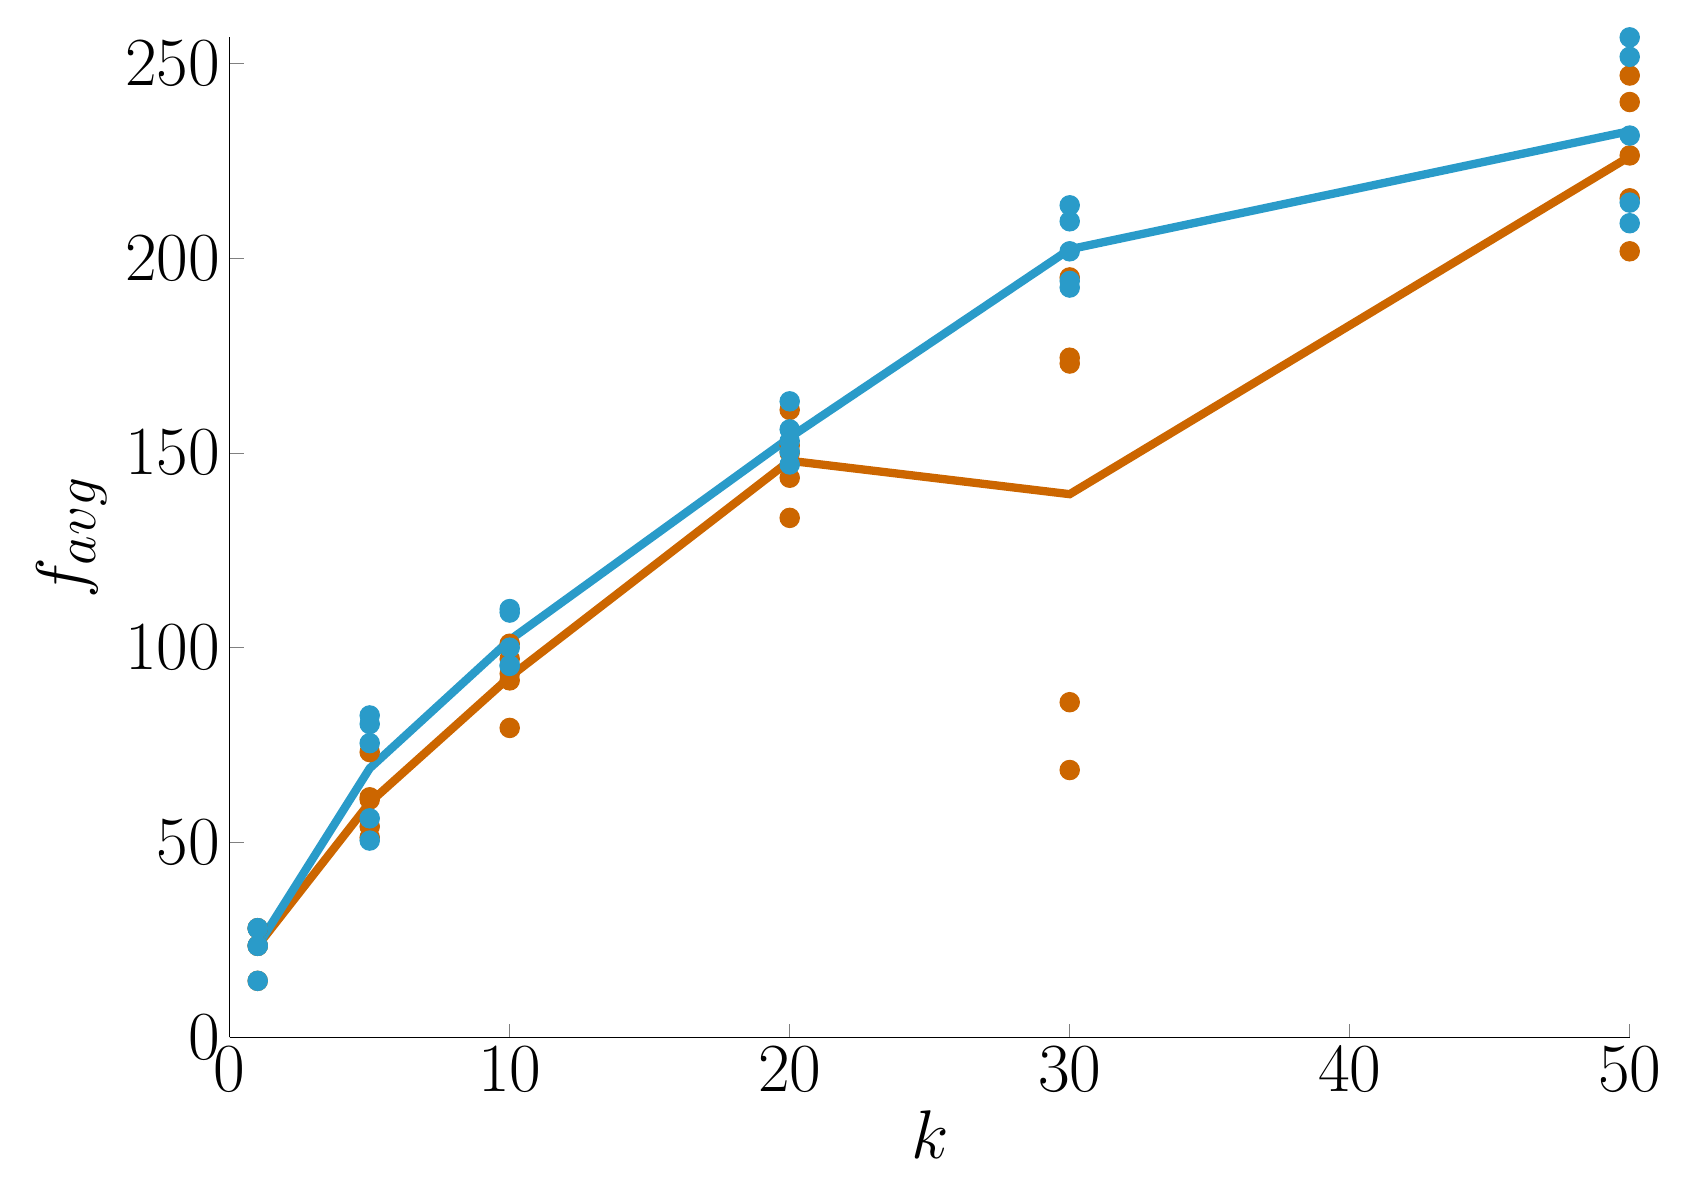
\begin{tikzpicture}

\begin{axis}[%
tick label style={font=\Huge},
label style={font=\Huge},
legend style={font=\Huge},
view={0}{90},
max space between ticks=50pt,
width=7in,
height=5in,
scale only axis,
xmin=0, xmax=50,
xtick={0, 10, 20, 30, 40, 50},
xlabel={$k$},
ymin=0, ymax=256.6,
%ytick={0, 200, 400, 600, 800, 1000},
ylabel={$f_{avg}$},
major tick length=5pt,
axis lines*=left,
legend cell align=left,
clip=false]

\addplot [
only marks,
mark=*,
mark size=3.5pt,
color=orange!80!black,
%solid,
%line width=2pt,
]
coordinates{
(1,14.5)(1,23.5)(1,23.5)(1,28.0)(1,28.0)(5,51.3)(5,54.1)(5,61.0)(5,61.6)(5,73.2)(10,79.4)(10,91.6)(10,93.3)(10,97.1)(10,101.0)(20,133.3)(20,143.6)(20,150.0)(20,151.9)(20,161.0)(30,68.6)(30,86.0)(30,172.9)(30,174.4)(30,195.0)(50,201.7)(50,215.3)(50,226.3)(50,240.0)(50,246.8)
};

\addplot [
only marks,
mark=*,
mark size=3.5pt,
color=cyan!80!black,
%solid,
%line width=2pt,
]
coordinates{
(1,14.5)(1,23.5)(1,23.5)(1,28.0)(1,28.0)(5,50.5)(5,56.2)(5,75.5)(5,80.4)(5,82.6)(10,95.3)(10,95.5)(10,100.0)(10,109.0)(10,109.9)(20,147.0)(20,150.3)(20,153.0)(20,156.0)(20,163.2)(30,192.4)(30,194.1)(30,201.7)(30,209.4)(30,213.5)(50,208.9)(50,214.2)(50,231.4)(50,251.6)(50,256.6)
};

\addplot [
color=orange!80!black,
solid,
line width=3pt
]
coordinates{
(1,23.5)(5,60.24)(10,92.48)(20,147.96)(30,139.38)(50,226.02)
};

\addplot [
color=cyan!80!black,
solid,
line width=3pt
]
coordinates{
(1,23.5)(5,69.04)(10,101.94)(20,153.9)(30,202.22)(50,232.54)
};


\end{axis}
\end{tikzpicture}
\end{document}
